% !TeX TXS-program:bibliography = txs:///biber
\documentclass[14pt, russian]{scrartcl}
\let\counterwithout\relax
\let\counterwithin\relax
%\usepackage{lmodern}
\usepackage{float}
\usepackage{xcolor}
\usepackage{extsizes}
\usepackage{subfig}
\usepackage[export]{adjustbox}
\usepackage{tocvsec2} % возможность менять учитываемую глубину разделов в оглавлении
\usepackage[subfigure]{tocloft}
\usepackage[newfloat]{minted}
\captionsetup[listing]{position=top}

\usepackage{fancyvrb}
\usepackage{ulem,bm,mathrsfs,ifsym} %зачеркивания, особо жирный стиль и RSFS начертание
\usepackage{sectsty} % переопределение стилей подразделов
%%%%%%%%%%%%%%%%%%%%%%%

%%% Поля и разметка страницы %%%
\usepackage{pdflscape}                              % Для включения альбомных страниц
\usepackage{geometry}                               % Для последующего задания полей
\geometry{a4paper,tmargin=2cm,bmargin=2cm,lmargin=3cm,rmargin=1cm} % тоже самое, но лучше

%%% Математические пакеты %%%
\usepackage{amsthm,amsfonts,amsmath,amssymb,amscd}  % Математические дополнения от AMS
\usepackage{mathtools}                              % Добавляет окружение multlined
\usepackage[perpage]{footmisc}
%\usepackage{times}

%%%% Установки для размера шрифта 14 pt %%%%
%% Формирование переменных и констант для сравнения (один раз для всех подключаемых файлов)%%
%% должно располагаться до вызова пакета fontspec или polyglossia, потому что они сбивают его работу
%\newlength{\curtextsize}
%\newlength{\bigtextsize}
%\setlength{\bigtextsize}{13pt}
\KOMAoptions{fontsize=14pt}

\makeatletter
\def\showfontsize{\f@size{} point}
\makeatother

%\makeatletter
%\show\f@size                                       % неплохо для отслеживания, но вызывает стопорение процесса, если документ компилируется без команды  -interaction=nonstopmode 
%\setlength{\curtextsize}{\f@size pt}
%\makeatother

%шрифт times
\usepackage{tempora}
%\usepackage{pscyr}
%\setmainfont[Ligatures={TeX,Historic}]{Times New Roman}

   %%% Решение проблемы копирования текста в буфер кракозябрами
%    \input glyphtounicode.tex
%    \input glyphtounicode-cmr.tex %from pdfx package
%    \pdfgentounicode=1
    \usepackage{cmap}                               % Улучшенный поиск русских слов в полученном pdf-файле
    \usepackage[T1]{fontenc}                       % Поддержка русских букв
    \usepackage[utf8]{inputenc}                     % Кодировка utf8
    \usepackage[english, main=russian]{babel}            % Языки: русский, английский
%   \IfFileExists{pscyr.sty}{\usepackage{pscyr}}{}  % Красивые русские шрифты
%\renewcommand{\rmdefault}{ftm}
%%% Оформление абзацев %%%
\usepackage{indentfirst}                            % Красная строка
%\usepackage{eskdpz}

%%% Таблицы %%%
\usepackage{longtable}                              % Длинные таблицы
\usepackage{multirow,makecell,array}                % Улучшенное форматирование таблиц
\usepackage{booktabs}                               % Возможность оформления таблиц в классическом книжном стиле (при правильном использовании не противоречит ГОСТ)

%%% Общее форматирование
\usepackage{soulutf8}                               % Поддержка переносоустойчивых подчёркиваний и зачёркиваний
\usepackage{icomma}                                 % Запятая в десятичных дробях



%%% Изображения %%%
\usepackage{graphicx}                               % Подключаем пакет работы с графикой
\usepackage{wrapfig}

%%% Списки %%%
\usepackage{enumitem}

%%% Подписи %%%
\usepackage{caption}                                % Для управления подписями (рисунков и таблиц) % Может управлять номерами рисунков и таблиц с caption %Иногда может управлять заголовками в списках рисунков и таблиц
%% Использование:
%\begin{table}[h!]\ContinuedFloat - чтобы не переключать счетчик
%\captionsetup{labelformat=continued}% должен стоять до самого caption
%\caption{}
% либо ручками \caption*{Продолжение таблицы~\ref{...}.} :)

%%% Интервалы %%%
\addto\captionsrussian{%
  \renewcommand{\listingname}{Листинг}%
}
%%% Счётчики %%%
\usepackage[figure,table,section]{totalcount}               % Счётчик рисунков и таблиц
\DeclareTotalCounter{lstlisting}
\usepackage{totcount}                               % Пакет создания счётчиков на основе последнего номера подсчитываемого элемента (может требовать дважды компилировать документ)
\usepackage{totpages}                               % Счётчик страниц, совместимый с hyperref (ссылается на номер последней страницы). Желательно ставить последним пакетом в преамбуле

%%% Продвинутое управление групповыми ссылками (пока только формулами) %%%
%% Кодировки и шрифты %%%

%   \newfontfamily{\cyrillicfont}{Times New Roman}
%   \newfontfamily{\cyrillicfonttt}{CMU Typewriter Text}
	%\setmainfont{Times New Roman}
	%\newfontfamily\cyrillicfont{Times New Roman}
	%\setsansfont{Times New Roman}                    %% задаёт шрифт без засечек
%	\setmonofont{Liberation Mono}               %% задаёт моноширинный шрифт
%    \IfFileExists{pscyr.sty}{\renewcommand{\rmdefault}{ftm}}{}
%%% Интервалы %%%
%linespread-реализация ближе к реализации полуторного интервала в ворде.
%setspace реализация заточена под шрифты 10, 11, 12pt, под остальные кегли хуже, но всё же ближе к типографской классике. 
\linespread{1.3}                    % Полуторный интервал (ГОСТ Р 7.0.11-2011, 5.3.6)
%\renewcommand{\@biblabel}[1]{#1}

%%% Гиперссылки %%%
\usepackage{hyperref}

%%% Выравнивание и переносы %%%
\sloppy                             % Избавляемся от переполнений
\clubpenalty=10000                  % Запрещаем разрыв страницы после первой строки абзаца
\widowpenalty=10000                 % Запрещаем разрыв страницы после последней строки абзаца

\makeatletter % малые заглавные, small caps shape
\let\@@scshape=\scshape
\renewcommand{\scshape}{%
  \ifnum\strcmp{\f@series}{bx}=\z@
    \usefont{T1}{cmr}{bx}{sc}%
  \else
    \ifnum\strcmp{\f@shape}{it}=\z@
      \fontshape{scsl}\selectfont
    \else
      \@@scshape
    \fi
  \fi}
\makeatother

%%% Подписи %%%
%\captionsetup{%
%singlelinecheck=off,                % Многострочные подписи, например у таблиц
%skip=2pt,                           % Вертикальная отбивка между подписью и содержимым рисунка или таблицы определяется ключом
%justification=centering,            % Центрирование подписей, заданных командой \caption
%}
%%%        Подключение пакетов                 %%%
\usepackage{ifthen}                 % добавляет ifthenelse
%%% Инициализирование переменных, не трогать!  %%%
\newcounter{intvl}
\newcounter{otstup}
\newcounter{contnumeq}
\newcounter{contnumfig}
\newcounter{contnumtab}
\newcounter{pgnum}
\newcounter{bibliosel}
\newcounter{chapstyle}
\newcounter{headingdelim}
\newcounter{headingalign}
\newcounter{headingsize}
\newcounter{tabcap}
\newcounter{tablaba}
\newcounter{tabtita}
%%%%%%%%%%%%%%%%%%%%%%%%%%%%%%%%%%%%%%%%%%%%%%%%%%

%%% Область упрощённого управления оформлением %%%

%% Интервал между заголовками и между заголовком и текстом
% Заголовки отделяют от текста сверху и снизу тремя интервалами (ГОСТ Р 7.0.11-2011, 5.3.5)
\setcounter{intvl}{3}               % Коэффициент кратности к размеру шрифта

%% Отступы у заголовков в тексте
\setcounter{otstup}{0}              % 0 --- без отступа; 1 --- абзацный отступ

%% Нумерация формул, таблиц и рисунков
\setcounter{contnumeq}{1}           % Нумерация формул: 0 --- пораздельно (во введении подряд, без номера раздела); 1 --- сквозная нумерация по всей диссертации
\setcounter{contnumfig}{1}          % Нумерация рисунков: 0 --- пораздельно (во введении подряд, без номера раздела); 1 --- сквозная нумерация по всей диссертации
\setcounter{contnumtab}{1}          % Нумерация таблиц: 0 --- пораздельно (во введении подряд, без номера раздела); 1 --- сквозная нумерация по всей диссертации

%% Оглавление
\setcounter{pgnum}{0}               % 0 --- номера страниц никак не обозначены; 1 --- Стр. над номерами страниц (дважды компилировать после изменения)

%% Библиография
\setcounter{bibliosel}{1}           % 0 --- встроенная реализация с загрузкой файла через движок bibtex8; 1 --- реализация пакетом biblatex через движок biber

%% Текст и форматирование заголовков
\setcounter{chapstyle}{1}           % 0 --- разделы только под номером; 1 --- разделы с названием "Глава" перед номером
\setcounter{headingdelim}{1}        % 0 --- номер отделен пропуском в 1em или \quad; 1 --- номера разделов и приложений отделены точкой с пробелом, подразделы пропуском без точки; 2 --- номера разделов, подразделов и приложений отделены точкой с пробелом.

%% Выравнивание заголовков в тексте
\setcounter{headingalign}{0}        % 0 --- по центру; 1 --- по левому краю

%% Размеры заголовков в тексте
\setcounter{headingsize}{0}         % 0 --- по ГОСТ, все всегда 14 пт; 1 --- пропорционально изменяющийся размер в зависимости от базового шрифта

%% Подпись таблиц
\setcounter{tabcap}{0}              % 0 --- по ГОСТ, номер таблицы и название разделены тире, выровнены по левому краю, при необходимости на нескольких строках; 1 --- подпись таблицы не по ГОСТ, на двух и более строках, дальнейшие настройки: 
%Выравнивание первой строки, с подписью и номером
\setcounter{tablaba}{2}             % 0 --- по левому краю; 1 --- по центру; 2 --- по правому краю
%Выравнивание строк с самим названием таблицы
\setcounter{tabtita}{1}             % 0 --- по левому краю; 1 --- по центру; 2 --- по правому краю

%%% Рисунки %%%
\DeclareCaptionLabelSeparator*{emdash}{~--- }             % (ГОСТ 2.105, 4.3.1)
\captionsetup[figure]{labelsep=emdash,font=onehalfspacing,position=bottom}

%%% Таблицы %%%
\ifthenelse{\equal{\thetabcap}{0}}{%
    \newcommand{\tabcapalign}{\raggedright}  % по левому краю страницы или аналога parbox
}

\ifthenelse{\equal{\thetablaba}{0} \AND \equal{\thetabcap}{1}}{%
    \newcommand{\tabcapalign}{\raggedright}  % по левому краю страницы или аналога parbox
}

\ifthenelse{\equal{\thetablaba}{1} \AND \equal{\thetabcap}{1}}{%
    \newcommand{\tabcapalign}{\centering}    % по центру страницы или аналога parbox
}

\ifthenelse{\equal{\thetablaba}{2} \AND \equal{\thetabcap}{1}}{%
    \newcommand{\tabcapalign}{\raggedleft}   % по правому краю страницы или аналога parbox
}

\ifthenelse{\equal{\thetabtita}{0} \AND \equal{\thetabcap}{1}}{%
    \newcommand{\tabtitalign}{\raggedright}  % по левому краю страницы или аналога parbox
}

\ifthenelse{\equal{\thetabtita}{1} \AND \equal{\thetabcap}{1}}{%
    \newcommand{\tabtitalign}{\centering}    % по центру страницы или аналога parbox
}

\ifthenelse{\equal{\thetabtita}{2} \AND \equal{\thetabcap}{1}}{%
    \newcommand{\tabtitalign}{\raggedleft}   % по правому краю страницы или аналога parbox
}

\DeclareCaptionFormat{tablenocaption}{\tabcapalign #1\strut}        % Наименование таблицы отсутствует
\ifthenelse{\equal{\thetabcap}{0}}{%
    \DeclareCaptionFormat{tablecaption}{\tabcapalign #1#2#3}
    \captionsetup[table]{labelsep=emdash}                       % тире как разделитель идентификатора с номером от наименования
}{%
    \DeclareCaptionFormat{tablecaption}{\tabcapalign #1#2\par%  % Идентификатор таблицы на отдельной строке
        \tabtitalign{#3}}                                       % Наименование таблицы строкой ниже
    \captionsetup[table]{labelsep=space}                        % пробельный разделитель идентификатора с номером от наименования
}
\captionsetup[table]{format=tablecaption,singlelinecheck=off,font=onehalfspacing,position=top,skip=-5pt}  % многострочные наименования и прочее
\DeclareCaptionLabelFormat{continued}{Продолжение таблицы~#2}
\setlength{\belowcaptionskip}{.2cm}
\setlength{\intextsep}{0ex}

%%% Подписи подрисунков %%%
\renewcommand{\thesubfigure}{\asbuk{subfigure}}           % Буквенные номера подрисунков
\captionsetup[subfigure]{font={normalsize},               % Шрифт подписи названий подрисунков (не отличается от основного)
    labelformat=brace,                                    % Формат обозначения подрисунка
    justification=centering,                              % Выключка подписей (форматирование), один из вариантов            
}
%\DeclareCaptionFont{font12pt}{\fontsize{12pt}{13pt}\selectfont} % объявляем шрифт 12pt для использования в подписях, тут же надо интерлиньяж объявлять, если не наследуется
%\captionsetup[subfigure]{font={font12pt}}                 % Шрифт подписи названий подрисунков (всегда 12pt)

%%% Настройки гиперссылок %%%

\definecolor{linkcolor}{rgb}{0.0,0,0}
\definecolor{citecolor}{rgb}{0,0.0,0}
\definecolor{urlcolor}{rgb}{0,0,0}

\hypersetup{
    linktocpage=true,           % ссылки с номера страницы в оглавлении, списке таблиц и списке рисунков
%    linktoc=all,                % both the section and page part are links
%    pdfpagelabels=false,        % set PDF page labels (true|false)
    plainpages=true,           % Forces page anchors to be named by the Arabic form  of the page number, rather than the formatted form
    colorlinks,                 % ссылки отображаются раскрашенным текстом, а не раскрашенным прямоугольником, вокруг текста
    linkcolor={linkcolor},      % цвет ссылок типа ref, eqref и подобных
    citecolor={citecolor},      % цвет ссылок-цитат
    urlcolor={urlcolor},        % цвет гиперссылок
    pdflang={ru},
}
\urlstyle{same}
%%% Шаблон %%%
%\DeclareRobustCommand{\todo}{\textcolor{red}}       % решаем проблему превращения названия цвета в результате \MakeUppercase, http://tex.stackexchange.com/a/187930/79756 , \DeclareRobustCommand protects \todo from expanding inside \MakeUppercase
\setlength{\parindent}{2.5em}                       % Абзацный отступ. Должен быть одинаковым по всему тексту и равен пяти знакам (ГОСТ Р 7.0.11-2011, 5.3.7).

%%% Списки %%%
% Используем дефис для ненумерованных списков (ГОСТ 2.105-95, 4.1.7)
%\renewcommand{\labelitemi}{\normalfont\bfseries~{---}} 
\renewcommand{\labelitemi}{\bfseries~{---}} 
\setlist{nosep,%                                    % Единый стиль для всех списков (пакет enumitem), без дополнительных интервалов.
    labelindent=\parindent,leftmargin=*%            % Каждый пункт, подпункт и перечисление записывают с абзацного отступа (ГОСТ 2.105-95, 4.1.8)
}
%%%%%%%%%%%%%%%%%%%%%%
%\usepackage{xltxtra} % load xunicode

\usepackage{ragged2e}
\usepackage[explicit]{titlesec}
\usepackage{placeins}
\usepackage{xparse}
\usepackage{csquotes}

\usepackage{listingsutf8}
\usepackage{url} %пакеты расширений
\usepackage{algorithm, algorithmicx}
\usepackage[noend]{algpseudocode}
\usepackage{blkarray}
\usepackage{chngcntr}
\usepackage{tabularx}
\usepackage[backend=biber, 
    bibstyle=gost-numeric,
    citestyle=nature]{biblatex}
\newcommand*\template[1]{\text{<}#1\text{>}}
\addbibresource{biblio.bib}
  
\titleformat{name=\section,numberless}[block]{\normalfont\Large\centering}{}{0em}{#1}
\titleformat{\section}[block]{\normalfont\Large\bfseries\raggedright}{}{0em}{\thesection\hspace{0.25em}#1}
\titleformat{\subsection}[block]{\normalfont\Large\bfseries\raggedright}{}{0em}{\thesubsection\hspace{0.25em}#1}
\titleformat{\subsubsection}[block]{\normalfont\large\bfseries\raggedright}{}{0em}{\thesubsubsection\hspace{0.25em}#1}

\let\Algorithm\algorithm
\renewcommand\algorithm[1][]{\Algorithm[#1]\setstretch{1.5}}
%\renewcommand{\listingscaption}{Листинг}

\usepackage{pifont}
\usepackage{calc}
\usepackage{suffix}
\usepackage{csquotes}
\DeclareQuoteStyle{russian}
    {\guillemotleft}{\guillemotright}[0.025em]
    {\quotedblbase}{\textquotedblleft}
\ExecuteQuoteOptions{style=russian}
\newcommand{\enq}[1]{\enquote{#1}}  
\newcommand{\eng}[1]{\begin{english}#1\end{english}}
% Подчиненные счетчики в окружениях http://old.kpfu.ru/journals/izv_vuz/arch/sample1251.tex
\newcounter{cTheorem} 
\newcounter{cDefinition}
\newcounter{cConsequent}
\newcounter{cExample}
\newcounter{cLemma}
\newcounter{cConjecture}
\newtheorem{Theorem}{Теорема}[cTheorem]
\newtheorem{Definition}{Определение}[cDefinition]
\newtheorem{Consequent}{Следствие}[cConsequent]
\newtheorem{Example}{Пример}[cExample]
\newtheorem{Lemma}{Лемма}[cLemma]
\newtheorem{Conjecture}{Гипотеза}[cConjecture]

\renewcommand{\theTheorem}{\arabic{Theorem}}
\renewcommand{\theDefinition}{\arabic{Definition}}
\renewcommand{\theConsequent}{\arabic{Consequent}}
\renewcommand{\theExample}{\arabic{Example}}
\renewcommand{\theLemma}{\arabic{Lemma}}
\renewcommand{\theConjecture}{\arabic{Conjecture}}
%\makeatletter
\NewDocumentCommand{\Newline}{}{\text{\\}}
\newcommand{\sequence}[2]{\ensuremath \left(#1,\ \dots,\ #2\right)}

\definecolor{mygreen}{rgb}{0,0.6,0}
\definecolor{mygray}{rgb}{0.5,0.5,0.5}
\definecolor{mymauve}{rgb}{0.58,0,0.82}
\renewcommand{\listalgorithmname}{Список алгоритмов}
\floatname{algorithm}{Листинг}
\renewcommand{\lstlistingname}{Листинг}
\renewcommand{\thealgorithm}{\arabic{algorithm}}

\newcommand{\refAlgo}[1]{(листинг \ref{#1})}
\newcommand{\refImage}[1]{(рисунок \ref{#1})}

\renewcommand{\theenumi}{\arabic{enumi}.}% Меняем везде перечисления на цифра.цифра	
\renewcommand{\labelenumi}{\arabic{enumi}.}% Меняем везде перечисления на цифра.цифра
\renewcommand{\theenumii}{\arabic{enumii}}% Меняем везде перечисления на цифра.цифра
\renewcommand{\labelenumii}{(\arabic{enumii})}% Меняем везде перечисления на цифра.цифра
\renewcommand{\theenumiii}{\roman{enumiii}}% Меняем везде перечисления на цифра.цифра
\renewcommand{\labelenumiii}{(\roman{enumiii})}% Меняем везде перечисления на цифра.цифра
%\newfontfamily\AnkaCoder[Path=src/fonts/]{AnkaCoder-r.ttf}
\renewcommand{\labelitemi}{---}
\renewcommand{\labelitemii}{---}

%\usepackage{courier}

\newenvironment{longlisting}{\captionsetup{type=listing}}{}

\makeatletter
\def\p@subsection{}
\def\p@subsubsection{\thesection\,\thesubsection\,}
\makeatother
\newcommand{\prog}[1]{{\ttfamily\small#1}}

\newcommand{\anonsection}[1]{\cleardoublepage
\phantomsection
\addcontentsline{toc}{section}{\protect\numberline{}#1}
\section*{#1}\vspace*{2.5ex} % По госту положены 3 пустые строки после заголовка ненумеруемого раздела
}
\newcommand{\sectionbreak}{\clearpage}
\renewcommand{\sectionfont}{\normalsize} % Сбиваем стиль оглавления в стандартный
\renewcommand{\cftsecleader}{\cftdotfill{\cftdotsep}} % Точки в оглавлении напротив разделов

\renewcommand{\cftsecfont}{\normalfont\large} % Переключение на times в содержании
\renewcommand{\cftsubsecfont}{\normalfont\large} % Переключение на times в содержании

\usepackage{caption} 
%\captionsetup[table]{justification=raggedleft} 
%\captionsetup[figure]{justification=centering,labelsep=endash}
\usepackage{amsmath}    % \bar    (матрицы и проч. ...)
\usepackage{amsfonts}   % \mathbb (символ для множества действительных чисел и проч. ...)
\usepackage{mathtools}  % \abs, \norm
    \DeclarePairedDelimiter\abs{\lvert}{\rvert} % операция модуля
    \DeclarePairedDelimiter\norm{\lVert}{\rVert} % операция нормы
\DeclareTextCommandDefault{\textvisiblespace}{%
  \mbox{\kern.06em\vrule \@height.3ex}%
  \vbox{\hrule \@width.3em}%
  \hbox{\vrule \@height.3ex}}    
\newsavebox{\spacebox}
\begin{lrbox}{\spacebox}
\verb*! !
\end{lrbox}
\newcommand{\aspace}{\usebox{\spacebox}}
\DeclareTotalCounter{listing}
    
\begin{document}
\sloppy

\def\figurename{Рисунок}

\begin{titlepage}
\thispagestyle{empty}
\newpage

\vspace*{-30pt}
\hspace{-45pt}
\begin{minipage}{0.17\textwidth}
\hspace*{-20pt}\centering
\includegraphics[width=1.3\textwidth]{emblem.png}
\end{minipage}
\begin{minipage}{0.82\textwidth}\small \textbf{
\vspace*{-0.7ex}
\hspace*{-10pt}\centerline{Министерство науки и высшего образования Российской Федерации}
\vspace*{-0.7ex}
\centerline{Федеральное государственное бюджетное образовательное учреждение }
\vspace*{-0.7ex}
\centerline{высшего образования}
\vspace*{-0.7ex}
\centerline{<<Московский государственный технический университет}
\vspace*{-0.7ex}
\centerline{имени Н.Э. Баумана}
\vspace*{-0.7ex}
\centerline{(национальный исследовательский университет)>>}
\vspace*{-0.7ex}
\centerline{(МГТУ им. Н.Э. Баумана)}}
\end{minipage}

\vspace{-2pt}
\hspace{-34.5pt}\rule{\textwidth}{2.5pt}

\vspace*{-20.3pt}
\hspace{-34.5pt}\rule{\textwidth}{0.4pt}
 
\vspace{0.5ex}
\noindent \small ФАКУЛЬТЕТ\hspace{80pt} <<Информатика и системы управления>>

\vspace*{-16pt}
\hspace{35pt}\rule{0.855\textwidth}{0.4pt}

\vspace{0.5ex}
\noindent \small КАФЕДРА\hspace{50pt} <<Теоретическая информатика и компьютерные технологии>>

\vspace*{-16pt}
\hspace{25pt}\rule{0.875\textwidth}{0.4pt}
 
 
\vspace{3em}
 
\begin{center}
\Large \bf{РАСЧЕТНО-ПОЯСНИТЕЛЬНАЯ ЗАПИСКА\\\textbf{\textit{К КУРСОВОЙ РАБОТЕ\\НА ТЕМУ:}} \\}
\end{center}

\vspace*{-6ex} 
\begin{center}
\Large{\textit{\textbf{<<Интерпретатор языка Scheme>>}}}

\vspace*{-3ex}
\rule{0.9\textwidth}{1.2pt}

\vspace*{-0.2ex}
\rule{0.9\textwidth}{1.2pt}

\vspace*{-0.2ex}
\rule{0.9\textwidth}{1.2pt}

\vspace*{-0.2ex}
\rule{0.9\textwidth}{1.2pt}

\vspace*{-0.2ex}
\rule{0.9\textwidth}{1.2pt}
\end{center}
 
\vspace{\fill}
 

\newlength{\ML}
\settowidth{\ML}{«\underline{\hspace{0.7cm}}» \underline{\hspace{2cm}}}

\noindent Студент \underline{ИУ9-72Б\hspace{1.5cm}} \hfill \underline{\hspace{4cm}}\quad
\underline{\hspace{0.3cm}А.Г. Владиславов\hspace{0.4cm}}

\vspace{-2.1ex}
\noindent\hspace{9ex}\scriptsize{(Группа)}\normalsize\hspace{170pt}\hspace{2ex}\scriptsize{(Подпись, дата)}\normalsize\hspace{30pt}\hspace{6ex}\scriptsize{(И.О. Фамилия)}\normalsize

\bigskip

\noindent Руководитель  \hfill \underline{\hspace{4cm}}\quad
\underline{\hspace{0.5cm}А.В. Синявин\hspace{0.5cm}}

\vspace{-2ex}
\noindent\hspace{13.5ex}\normalsize\hspace{170pt}\hspace{2ex}\scriptsize{(Подпись, дата)}\normalsize\hspace{30pt}\hspace{6ex}\scriptsize{(И.О. Фамилия)}\normalsize
\vfill

%\vspace{\fill}
 


\begin{center}
\textsl{2022 г.}
\end{center}
\end{titlepage}

%\renewcommand{\ttdefault}{pcr}

\setlength{\tabcolsep}{3pt}
\newpage
\setcounter{page}{2}
%----------------------------------------------------------------------------
%                  ОТСЮДА --- СОБСТВЕННО ТЕКСТ
%----------------------------------------------------------------------------

\renewcommand\contentsname{\hfill{\normalfont{СОДЕРЖАНИЕ}}\hfill}  %Оглавление
\tableofcontents
\newpage
\anonsection{ВВЕДЕНИЕ}  %Введение

Цель данной работы - реализация большой части функций интерпретатора подмножества R$^5$RS языка Scheme.

Программа интерпретатора должна считывать из потока ввода или из текстового файла код на языке Scheme и выдавать результат работы данной программы.

Необходимо изучить спецификации языка для написания интерпретатора.

Также необходимо изучить инструменты для написания легко масштабируемого и переносимого под разные платформы программного кода, с целью дальнейшего развития интерпретатора.

На основе изученных данных необходимо написать интерпретатор.

\section{Постановка задачи, обзор технологий}

Задачей данной работы было выбрано написание интерпретатора языка Scheme --- функционального языка программирования, одного из наиболее популярных диалектов Lisp. На кафедре ИУ9 данный язык изучается на первом семестре первого курса, так что базовое понимание уже присутствует

\subsection{Обзор интерпретируемого языка}

В рамках курсовой будет разобрана большая часть стандарта R$^5$RS языка Scheme, описанного в документе ~\cite{R5rs}. Из данного стандарта будет реализован основной набор функций языка, чтобы на нём была возможность запускать лабораторные работы, выполняемые на первом курсе. Реализованные функции языка были поделены на категории, представленнив в таблице ~\ref{tab:functions}.

\bigskip

\begin{table}[htb]
\caption{\centering Релизованные функции языка.}
\small
\begin{tabular}{|c|c|c|}

\hline
\multicolumn{1}{|c|}{Категория}   & \multicolumn{1}{c|}{Функции, относящиеся к катеригии}                                                                                                                                         \\ \hline
Операции с числами                & +, -, *, /, number?                                                                                                                                                                           \\ \hline
Операции с логическими значениями & not, boolean?                                                                                                                                                                                 \\ \hline
Операции с символами              & char?                                                                                                                                                                                         \\ \hline
Операции со строками              & string?                                                                                                                                                                                       \\ \hline
Операции с символами              & symbol?                                                                                                                                                                                       \\ \hline
Равенства и неравенства           & eq?, eqv?, \textgreater{}, \textless{}                                                                                                                                                        \\ \hline
Операции с парами и списками      & car, cdr, cons, list, pair?, null?, set-car!, set-cdr!,                                                                                                                                       \\ \hline
Синтаксические операции           & \begin{tabular}[c]{@{}l@{}}quote, quasiquote, define, lambda, if, set!,\\ begin, cond, else\end{tabular}                                                                                      \\ \hline
Системный интерфейс               & load                                                                                                                                                                                          \\ \hline
Ввод                              & eof-object?, read                                                                                                                                                                             \\ \hline
Вывод                             & display, write, newline, flush,                                                                                                                                                               \\ \hline
Операции с портами ввода/вывода   & \begin{tabular}[c]{@{}l@{}}port?, input-port?, output-port?, textual-port?,\\ binary-port?, current-input-port, current-output-port\end{tabular}                                              \\ \hline
Вычисление                        & \begin{tabular}[c]{@{}l@{}}eval, null-environment, scheme-report-environment,\\  interaction-environment, current-environment, \\ in-environment, make-environment, environment?\end{tabular} \\ \hline
Функции управления                & call-with-current-continuation, procedure?, apply                                                                                                                                             \\ \hline

\end{tabular}
\label{tab:functions}
\end{table}

В листинге~\ref{lst:schemebnf} представлено описание грамматики языка Scheme в форме Бэкуса-Наура

\begin{listing}[!htb]
\caption{Описание грамматики языка Scheme в форме Бэкуса-Наура}
\label{lst:schemebnf}
\begin{minted}[frame=single,fontsize = \footnotesize, linenos, breaklines, xleftmargin = 1.5em,breaksymbol = ""]{BNF}
<program> ::= <expression>
<expression> ::= <constant> | <variable> | <procedure-call> | <conditional> | <lambda> | <definition>
<constant> ::= <number> | <boolean> | <string> | <char> | <symbol>
<number> ::= [0-9]+
<boolean> ::= #t | #f
<string> ::= ".*"
<char> ::= #\\.
<symbol> ::= [a-zA-Z]+
<variable> ::= [a-zA-Z]+
<procedure-call> ::= (<procedure> <expression>*)
<procedure> ::= + | - | * | / | number? | not | boolean? | char? | string? | symbol? | eq? | eqv? | > | < | car | cdr | cons | list | pair? | null? | set-car! | set-cdr! | quote | quasiquote | define | lambda | if | set! | begin | cond | else | load | eof-object? | read | display | write | newline | flush | port? | input-port? | output-port? | textual-port? | binary-port? | current-input-port | current-output-port | eval | null-environment | scheme-report-environment | interaction-environment | current-environment | in-environment | make-environment | environment? | call-with-current-continuation | procedure? | apply
<conditional> ::= (if <predicate> <expression> <expression>)
	| (cond (<predicate> <expression>)+ [else <expression>])
<predicate> ::= <expression>
<lambda> ::= (lambda (<variable>*) <expression>)
<definition> ::= (define <variable> <expression>)
\end{minted}
\end{listing}

\subsection{Выбор языка для написания интерпретатора}

Для реализации интерпретатора было желание выбрать популярный язык, программный код на котором на котором возможно собрать на большинстве операционных систем, настройка окружения не должна занимать много времени, была возможность легко расширять программу и впоследствии написать графический пользовательский интерфейс для взаимодействия не только через командную строку.
К данному описанию подходит язык Kotlin~\cite{Kotlindocs} --- современный язык, разрабатываемый компанией JetBrains.
Данный язык широко используется при разработке мобильных приложений.
Помимо JVM, данный язык имеет LLVM и JS бэкенды компилятора, что значительно расширяет области применения, благодаря чему, при определенных модификациях программного кода (избавления от зависимостей Java) интерпретатор можно использовать не только для на персональном компьютере, но и на мобильных устройствах~\cite{Kmm}, на сервере~\cite{Kserv} и в веб-страницах браузера~\cite{Kjs}.


\section{Проектирование программного комплекса}

Программа должна представлять из себя интерфейс командной строки.
На вход пользователь вводит программный код на языке Scheme, на выход получает результат интерпретации введённого кода.

Программа состоит лексического анализатора, разбивающего входной текст на лексемы, синтаксического анализатора, составляющий дерево разбора и интерпретатора, обрабатывающего разобранное дерево и выполняющего код.

На рисунке~\ref{fig::parse} представлен пример разбора простого арифметического выражения на языке Scheme.


\begin{figure}[!htb]\centering
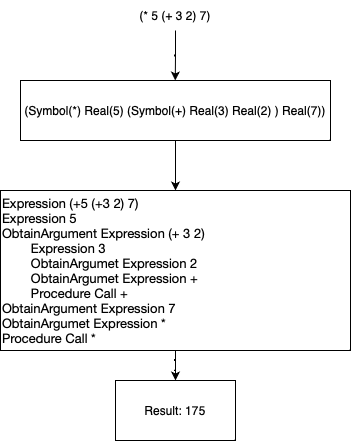
\includegraphics[width=0.5\textwidth]{parse.png}
\caption{Пример разбора арифметического выражения.}
\label{fig::parse}
\end{figure}

\section{Разработка программного комплекса}

\subsection{Базовые элементы для сущностей}

Для всех сущностей интерпретатора был создан интерфейс с набором методов, которые должны быть реализованы во всех наследниках интерфейса.
Список методов представлен в листинге~\ref{lst:entitykt}.

\begin{listing}[!htb]
\caption{Базовый интерфейс Entity}
\label{lst:entitykt}
\begin{minted}[frame=single,fontsize = \footnotesize, linenos, breaklines, xleftmargin = 1.5em,breaksymbol = ""]{kotlin}
interface Entity : Serializable {

    fun eval(env: Environment, continuation: Continuation): Entity?

    fun analyze(env: Environment): Entity

    fun optimize(env: Environment): Entity

    fun write(out: PrintWriter)

    fun display(out: PrintWriter)

    fun toWriteFormat(): String

    override fun toString(): String
}
\end{minted}
\end{listing}

Интерфейс \texttt{Entity} реализуется в классе \texttt{AbstractEntity}, от которого наследуются практически все сущности в программном коде интерпретатора (помимо списков). В данном классе представлены базовые реализации методов интерфейса. Код данного класса представлен в листинге ~\ref{lst:abstentkt}.

\begin{listing}[!htb]
\caption{Класс AbstractEntity}
\label{lst:abstentkt}
\begin{minted}[frame=single,fontsize = \footnotesize, linenos, breaklines, xleftmargin = 1.5em,breaksymbol = ""]{kotlin}
abstract class AbstractEntity : Entity {
    override fun eval(env: Environment, continuation: Continuation): Entity? = this

    override fun analyze(env: Environment): Entity = this

    override fun optimize(env: Environment): Entity = this

    override fun display(out: PrintWriter) {
        write(out)
    }

    override fun toWriteFormat(): String {
        val sw = StringWriter()
        display(PrintWriter(sw))
        return sw.toString()
    }

    override fun toString(): String {
        val sw = StringWriter()
        display(PrintWriter(sw))
        return sw.toString()
    }
}

\end{minted}
\end{listing}

Также интерфейс \texttt{Entity} наследуется в интерфейсе: \texttt{List}.
Данный интерфейс отвечает за последовательности сущностей и помимо \texttt{Entity} также реализует интерфейс \texttt{Iterable} для итерации по элементам списка, внутри себя имеет два поля: \texttt{car} и \texttt{cdr}, отвечающие за первый и последующие элменты списка.
Код \texttt{List} представлен в листинге~\ref{lst:listkt}.

\begin{listing}[!htb]
\caption{Интерфейс List}
\label{lst:listkt}
\begin{minted}[frame=single,fontsize = \footnotesize, linenos, breaklines, xleftmargin = 1.5em,breaksymbol = ""]{kotlin}
interface List : Entity, Iterable<Entity?> {
    var car: Entity
    var cdr: Entity
}
\end{minted}
\end{listing}

\subsection{Действия над сущностями}

Для действий был создан базовый класс \texttt{Action}.
Данный класс выполняет различные действия с сущностями и имеет ссылку на следующее действие.
Код данного класса представлен в листинге~\ref{lst:actionkt}

\begin{listing}[!htb]
\caption{Класс Action}
\label{lst:actionkt}
\begin{minted}[frame=single,fontsize = \footnotesize, linenos, breaklines, xleftmargin = 1.5em,breaksymbol = ""]{kotlin}
abstract class Action(
    val env: Environment?,
    var next: Action?,
) : Serializable {

    fun andThen(action: Action): Action {
        action.next = this.next
        this.next = action
        return action
    }

    abstract fun invoke(arg: Entity, cont: Continuation): Entity?

    protected fun interface Printer {
        fun print(port: OutputPort)
    }

    protected fun trace(doo: Printer, env: Environment?) {
        if (env?.interpreter?.traceEnabled == true) {
            val cout = env.out ?: return
            val actionName = this.javaClass.simpleName.replace("Action", "")
            cout.printf("%s ", actionName)
            doo.print(cout)
        }
    }
}

\end{minted}
\end{listing}

Данный абстрактный класс наследуется семью другими для реализации действий.

В данной релизации интерпретатора представлено 7 действий: \texttt{AssignmentAction}, \texttt{EvalAction}, \texttt{ExpressionAction}, \texttt{ExpressionInEnvAction}, \texttt{IfAction}, \texttt{ObtainArgumentAction}, \texttt{ProcedureCallAction}.
В листинге~\ref{lst:actionsimplkt} представлены реализации метода \texttt{invoke} для разных действий.

\begin{longlisting}[!htb]
\caption{Реализация метода \texttt{invoke} для различных действий}
\label{lst:actionsimplkt}
\begin{minted}[frame=single,fontsize = \footnotesize, linenos, breaklines, xleftmargin = 1.5em,breaksymbol = ""]{kotlin}
// Assignment --- операция присваивания
override fun invoke(arg: Entity, cont: Continuation): Entity? {
    cont.head = next
    env?.getLocation(symbol)!!.value = arg
    trace({ out -> out.print("${symbol.toWriteFormat()} <- ${arg.toWriteFormat()}\n") }, env)
    return Void.VALUE
}
// Eval --- операция вычисления
override fun invoke(arg: Entity, cont: Continuation): Entity? {
    cont.head = next
    trace({ out -> out.print("${arg.toWriteFormat()}\n") }, env)
    return arg.eval(env ?: return null, cont)
}
// Expression --- вычисление выражения
override fun invoke(arg: Entity, cont: Continuation): Entity? {
    cont.head = next
    trace({ port -> port.printf("${expr.toWriteFormat()}\n") }, env)
    return expr.eval(env ?: return null, cont)
}
// ExpressionInEnv --- вычисление выражения в определенном окружении
override fun invoke(arg: Entity, cont: Continuation): Entity? {
    cont.head = next
    if (arg !is Environment) {
        throw Exception("Not an environment $arg")
    }
    val evalEnv = arg
    expr = expr.analyze(evalEnv).optimize(evalEnv)
    trace({ out -> out.print("${expr.toWriteFormat()}\n") }, env)
    return expr.eval(evalEnv, cont)
}
// If --- условный оператор. Реализация также имеет поля consequent и alternate
override fun invoke(arg: Entity, cont: Continuation): Entity? {
    cont.head = next
    return if (arg != KSBoolean.FALSE) {
        consequent.eval(env ?: throw Exception("Null env"), cont)
    } else {
        alternate.eval(env ?: throw Exception("Null env"), cont)
    }
}
// ObtainArgument --- получение аргумента выражения
override fun invoke(arg: Entity, cont: Continuation): Entity? {
    cont.head = next
    argList.set(argumentIndex, arg)
    trace({ out -> out.print("") }, env)
    return arg
}
// ProcedureCall --- выполнение процедуры
override fun invoke(arg: Entity, cont: Continuation): Entity? {
    cont.head = next
    val operator: Procedure = arg as? Procedure ?: throw Exception("Operator not a procedure")
    trace({ out -> out.print("${arg.toWriteFormat()}\n") }, env)
    return operator.apply(argList.getArgs(), env!!, cont)
}
\end{minted}
\end{longlisting} % $
\subsection{Примитивные процедуры}

Для примитивных процедур был написан абстрактный класс \texttt{Primitives}, расположенный в пакете \texttt{lib}.
Этот класс имеет поля:
\begin{itemize} % or enumerate
\item \texttt{name} --- имя, как в программе;
\item \texttt{definitionEnv} --- окружение, в котором используется примитив;
\item \texttt{keyword} --- флаг, показывающий, является примитив частью синтаксиса;
\item \texttt{minArgs} --- минимальное число аргументов для использования примитива;
\item \texttt{maxArgs} --- максимальное число аргументов для использования примитива;
\item \texttt{comment} --- короткая заметка о примитиве;
\item \texttt{documentation} --- опциональное поле, более долгое объяснение, возможно с примером использования;
\end{itemize}

Также, поскольку большинство примитивов имеют ограниченное количество параметров для выполнения, этот класс имеет методы \texttt{apply0}, \texttt{apply1}, \texttt{apply2}, \texttt{apply3}, \texttt{applyN} --- для выполнения процедуры с определённым количеством параметров.

\subsection{Чтение и запись в консоль}

На данном этапе программа должна представлять себа консольную утилиту, принимающую на вход набор команд на языке Scheme, интерпретирующую их и выдающую результат работы программы в вывод. Для ввода и вывода используются стандартные Java интерфейсы для чтения и записи в консоль (\texttt{java.io.Reader}, \texttt{java.io.PrintWriter}). Для более удобной работы с вводом и выводом были написаны классы - \texttt{InputPort} и \texttt{OutputPort}, наследуемые от базового абстрактного класса \texttt{Port}.

Для разбиения на токены используется класс \texttt{Reader}, который, в свою очередь использует \texttt{java.io.StreamTokenizer}.
В листинге~\ref{lst:readerinit} представлен код инициализации класса \texttt{Reader}, в  котором указываются интервалы для различных категорий токенов.

\begin{listing}[!htb]
\caption{Инициализация класса \texttt{Reader}}
\label{lst:readerinit}
\begin{minted}[frame=single,fontsize = \footnotesize, linenos, breaklines, xleftmargin = 1.5em,breaksymbol = ""]{kotlin}
init {
    tokenizer.resetSyntax()
    tokenizer.lowerCaseMode(false)
    tokenizer.slashStarComments(false)
    tokenizer.commentChar(';'.code)
    tokenizer.quoteChar('\"'.code)
    tokenizer.whitespaceChars('\u0000'.code, '\u0020'.code)
    tokenizer.eolIsSignificant(false)
    tokenizer.wordChars('A'.code,'Z'.code) // A-Z
    tokenizer.wordChars('a'.code,'z'.code) // a-z
    tokenizer.wordChars('0'.code,'9'.code) // 0-9
    tokenizer.wordChars('\u00A1'.code,'\u00FF'.code) // Unicode latin-1 supplement, symbols and letters
    tokenizer.wordChars('*'.code,'.'.code) // '*', '+', ',', '-', '.'
    tokenizer.wordChars('!'.code,'!'.code) // '!'
    tokenizer.wordChars('#'.code, '#'.code)
    tokenizer.wordChars('\\'.code,'\\'.code) // '\'
    tokenizer.wordChars('/'.code,'/'.code) // '/'
    tokenizer.wordChars('$'.code,'$'.code) // '$' $
    tokenizer.wordChars('_'.code,'_'.code) // '_'
    tokenizer.wordChars('<'.code,'@'.code) // '<', '=', '>', '?', '@'
}
\end{minted}
\end{listing}

Непосредственно чтение токенов происходи в методе \texttt{readToken}, представленном в листинге~\ref{lst:readtoken}.

\begin{listing}[!htb]
\caption{Чтение токенов в классе \texttt{Reader}}
\label{lst:readtoken}
\begin{minted}[frame=single,fontsize = \footnotesize, linenos, breaklines, xleftmargin = 1.5em,breaksymbol = ""]{kotlin}
private fun readToken(): String? {
    val c = tokenizer.nextToken()
    return when (tokenizer.ttype) {
        StreamTokenizer.TT_EOF -> null
        StreamTokenizer.TT_NUMBER -> tokenizer.nval.toString()
        StreamTokenizer.TT_WORD -> tokenizer.sval
        '\"'.code -> "\"${tokenizer.sval}"
        else -> c.toChar().toString()
    }.also {
        if (it != null) {
            Logger.log(Logger.Level.DEBUG, "TOKEN=$it")
        }
    }
}
\end{minted}
\end{listing}

Далее происходит разбор в методе \texttt{readObject}, представленном в листинге~\ref{lst:readobject}.

\begin{listing}[!htb]
\caption{Реализация метода \texttt{readObject}}
\label{lst:readobject}
\begin{minted}[frame=single,fontsize = \footnotesize, linenos, breaklines, xleftmargin = 1.5em,breaksymbol = ""]{kotlin}
private fun readObject(token: String): Entity? {
    if (token.isEmpty()) {
        return readObject()
    }
    when (token) {
        "(" -> {
            return readList(Pair(car = EmptyList.VALUE, cdr = EmptyList.VALUE))
        }
        "'" -> { return Pair(car = Symbol.QUOTE, Pair(car = readObject() ?: return null, cdr = EmptyList.VALUE)) }
        "`" -> { return Pair(car = Symbol.QUASIQUOTE, Pair(car = readObject() ?: return null, cdr = EmptyList.VALUE)) }
        ")" -> { throw Exception("Unexpected \")\"") }
        else -> { return readOthers(token) }
    }
}
\end{minted}
\end{listing}

\subsection{Чтение из файла}

Некоторые функции языка были взяты из документа prelude.scheme~\cite{UMBScheme} --- файла, разработанного для инициализации языка Scheme стандарта R4RS, разработанного в университете Массачусетса в Бостоне в 1990 году.
В данном файле описаны многие функции, которые возможно реализовать на базе написанного в интерпретаторе кода. Данный файл загружается в интерпретатор при его инициализации, в функции, представленной в листинге~\ref{lst:bootstrap}.
Файл \texttt{bootstrap.scm} находится в ресурсах, используемых программой.

\begin{listing}[!htb]
\caption{Чтение файла для инициализации некоторых функций}
\label{lst:bootstrap}
\begin{minted}[frame=single,fontsize = \footnotesize, linenos, breaklines, xleftmargin = 1.5em,breaksymbol = ""]{kotlin}
fun bootstrap() {
    if (!bootstrapped) {
        val bootstrap = InputPort(
            BufferedReader(
                InputStreamReader(
                    javaClass.getResourceAsStream("/bootstrap.scm") ?: throw Exception("file null")
                )
            )
        )
        load(bootstrap, reportEnv)
    }
}
\end{minted}
\end{listing}

Функция \texttt{load} считывает исходный код из файла, на данный момент в коде она использьуется только для инициализации, но на её основе была написана функция, используемая для тестирования, которая будет разобрана в соответствующем разделе.

\subsection{Итоговая диаграмма классов}

На рисунке~\ref{fig::diagram} представлена итоговая диаграмма классов программного комплекса.

\begin{figure}[!htb]\centering
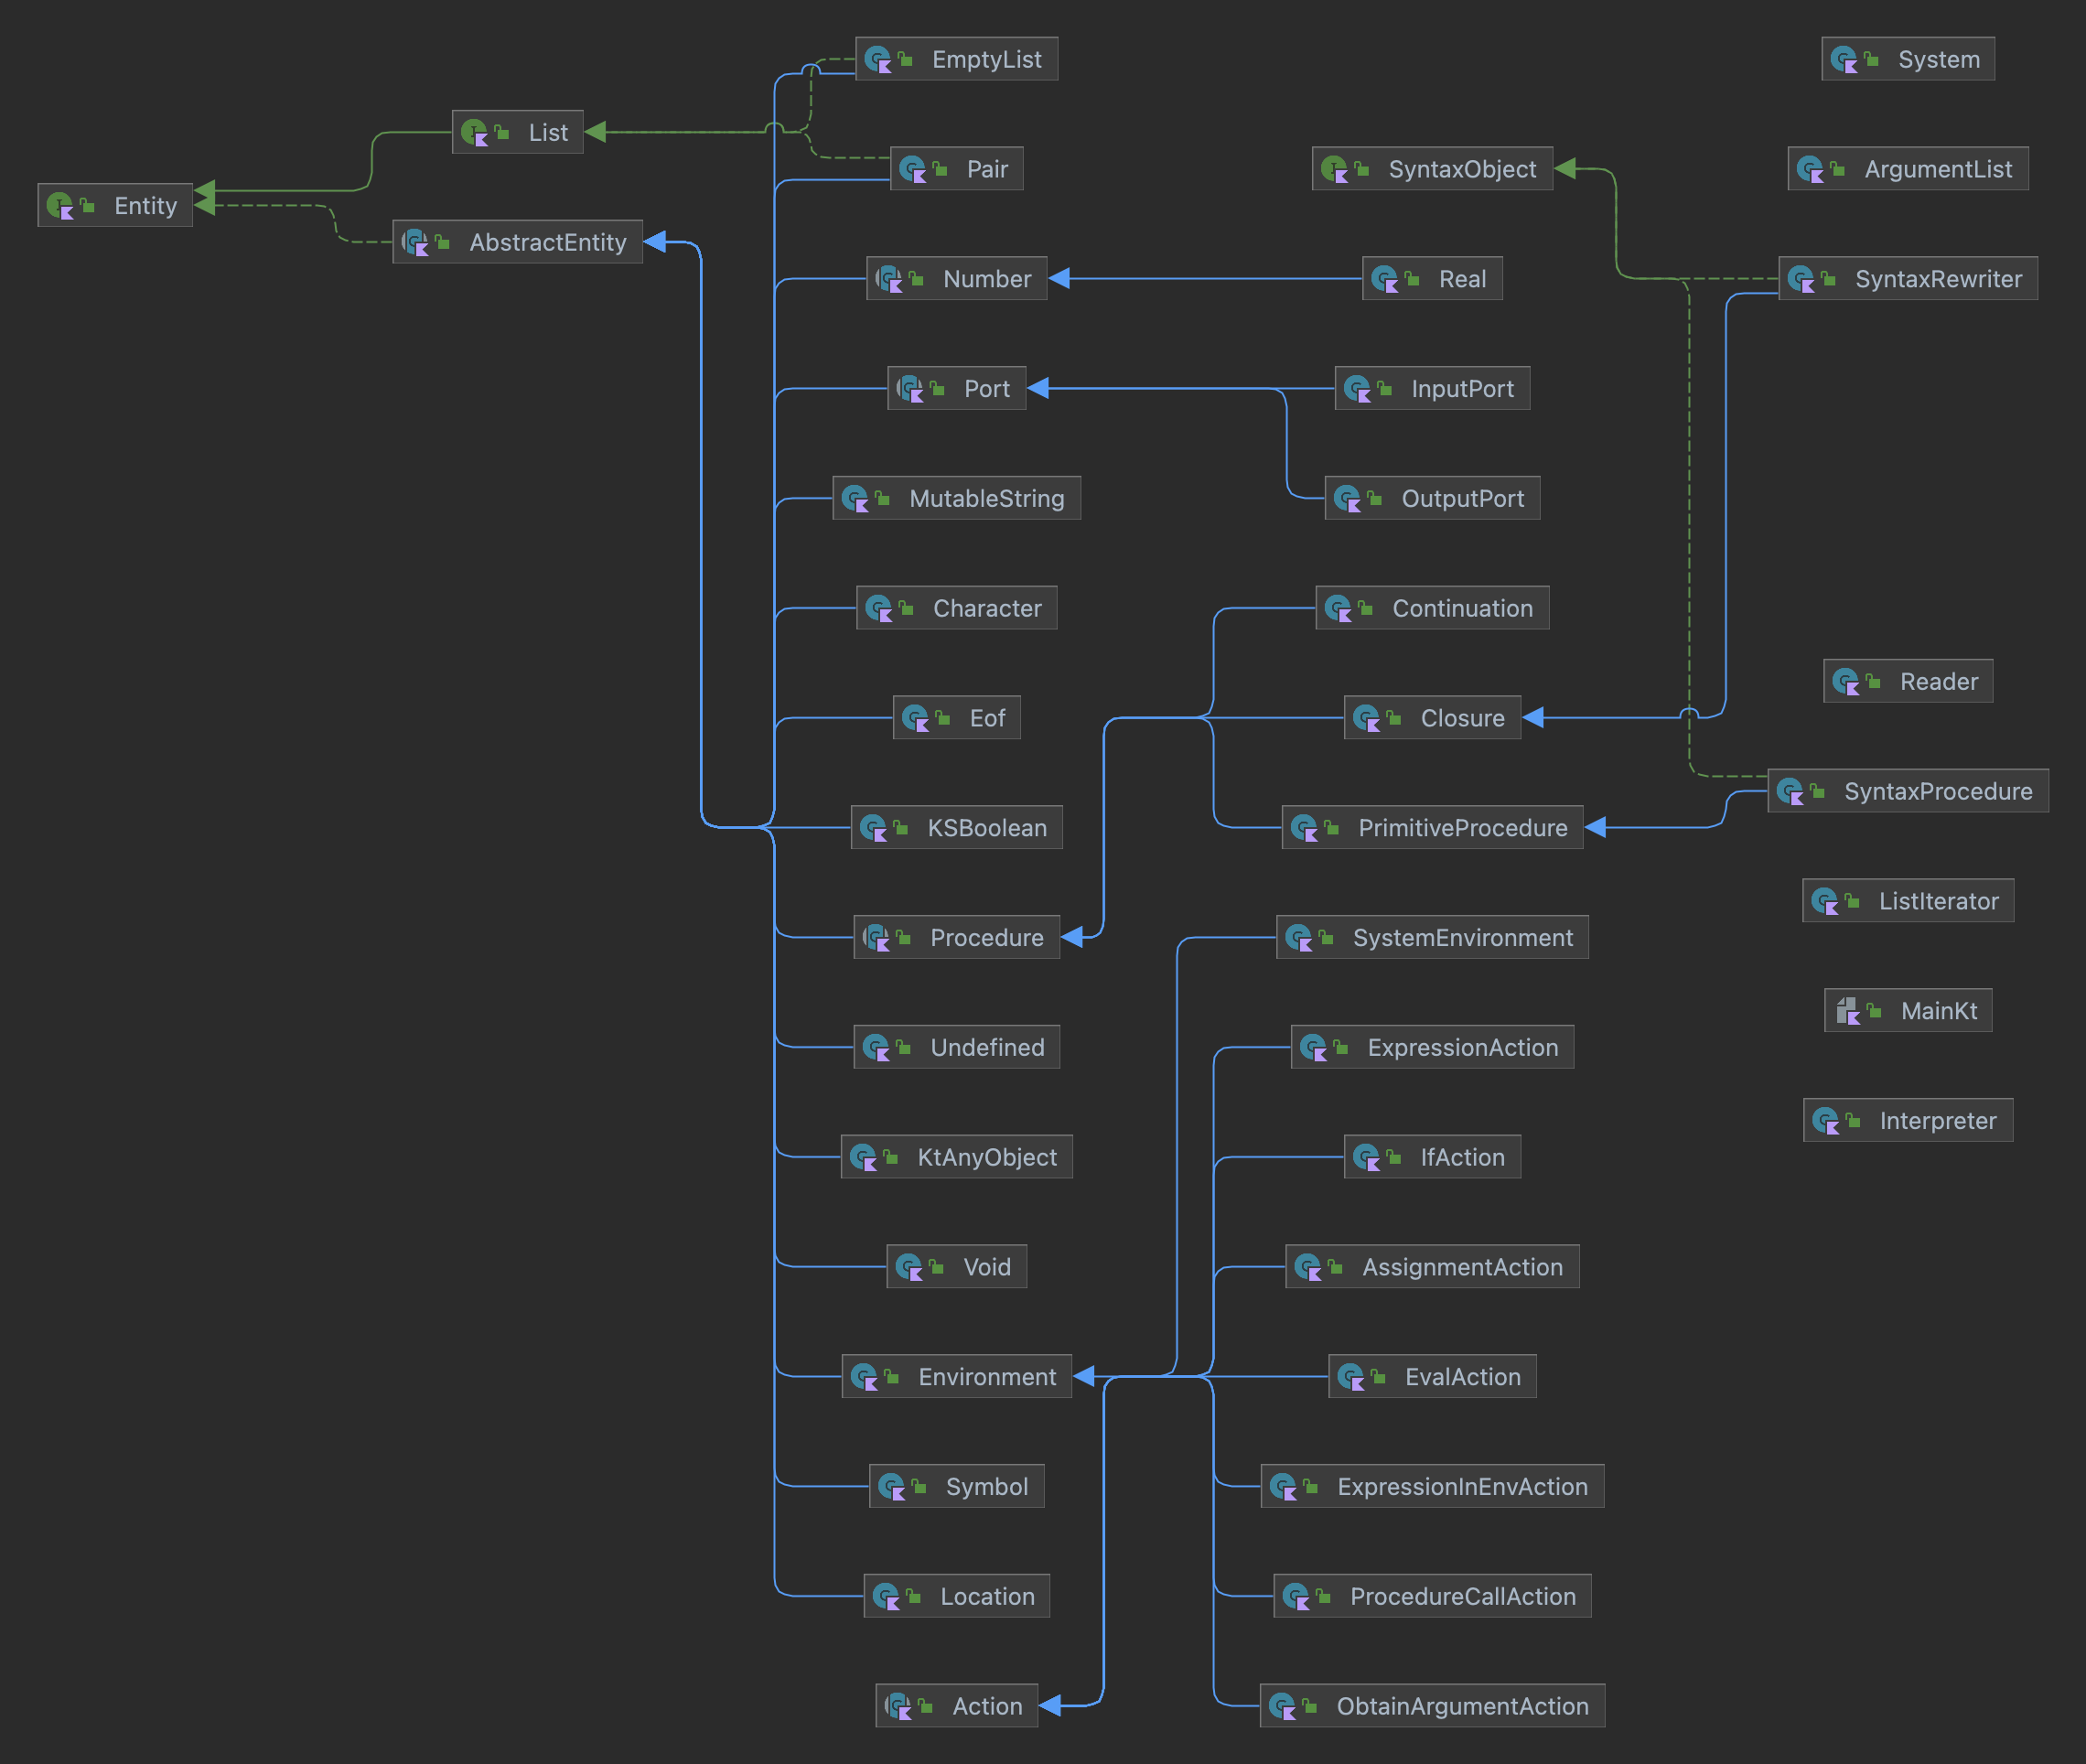
\includegraphics[width=0.5\textwidth]{diagram.png}
\caption{Диаграмма классов программного комплекса.}
\label{fig::diagram}
\end{figure}

\section{Тестирование программного комплекса}

\subsection{Тесты}

Для проверки работоспособности и корректности работы интерпретатора, был написан ряд unit-тестов, покрывающих основной функционал интерпретатора.
Помимо основных проверок, таких как операции сложения, вычитания, умножения, деления, сравнения, операций со списками и так далее, был написан пример интерпретатора на языке Scheme, который должен быть разобран и запущен интерпретатором, написанным в рамках данной работы.
Для проверки корректности тестов одни и те же фрагменты кода запускались "основным" интерпретатором и интерпретатором, используемом для тестирования.
В листинге ~\ref{lst:intptscm} представлен исходный код на языке Scheme, используемый для тестирования, в листинге~\ref{lst:testrun} представлен код для запуска теста

\begin{longlisting}
\caption{Интерпретатор для тестирования программного комплекса}
\label{lst:intptscm}
\begin{minted}[frame=single,fontsize = \footnotesize, linenos, breaklines, xleftmargin = 1.5em,breaksymbol = ""]{scheme}
(define (evlis exprs)
    (if (null? exprs)
        '()
        (cons (evaluate (car exprs)) (evlis (cdr exprs)) )))

(define (from-racket-bool x)
    (if x 't 'f))

(define (to-racket-bool x)
    (cond ((eq? x 't) #t)
          ((eq? x 'f) #f)
          (else (error 'to-racket-bool "not t or f"))))

(define (evaluate expr)
  (cond ((number? expr) expr)
    ((eq? (car expr) 'quote) (cadr expr))
    ((eq? (car expr) 'if) (if (to-racket-bool (evaluate (cadr expr)))
                            (evaluate (caddr expr))
                            (evaluate (cadddr expr))))
    (else (apply-fun (car expr) (evlis (cdr expr))))))
                            
(define (apply-fun fun xs)
    (cond ((eq? fun '*) (* (car xs) (cadr xs)))
          ((eq? fun '+) (+ (car xs) (cadr xs)))
          ((eq? fun '-) (- (car xs) (cadr xs)))
          ((eq? fun '/) (/ (car xs) (cadr xs)))
          
          ((eq? fun 'car) (caar xs))
          ((eq? fun 'cdr) (cdar xs))
          ((eq? fun 'cons) (cons (car xs) (cadr xs)))
          
          ((eq? fun 'list) xs)
          ((eq? fun 'null?) (from-racket-bool (null? (car xs))))))
\end{minted}
\end{longlisting}

\begin{longlisting}

\caption{Код для тестирования интерпретатора}
\label{lst:testrun}
\begin{minted}[frame=single,fontsize = \footnotesize, linenos, breaklines, xleftmargin = 1.5em,breaksymbol = ""]{kotlin}
class SchemeInterpretTest {
    lateinit var interpreter: Interpreter

    @BeforeTest
    fun init() {
        interpreter = Interpreter.newInterpreter()
        val inputPort = InputPort(
            BufferedReader(
                InputStreamReader(
                    javaClass.getResourceAsStream("/scheme/scheme-interpreter.scm") ?: throw Exception("file null")
                )
            )
        )
        interpreter.loadForTest(inputPort, interpreter.sessionEnv!!)
    }

    @Test
    fun runTest() {
        val expr = "(if (null? '(a b c)) 'a 'b)"
        run(expr)
    }

    @Test
    fun runTest2() {
        val expr = "(* (+ 2 3) (- 10 2))"
        run(expr)
    }

    @Test
    fun runTest3() {
        val expr = "(car (cdr (quote (a b c))))"
        run(expr)
    }

    @Test
    fun runTest4() {
        val expr = "(cons (+ 1 7) '(b c d))"
        run(expr)
    }

    @Test
    fun runTest5() {
        val expr = "(list (+ 3 9) (* 5 6))"
        run(expr)
    }

    private fun run(expr: String) {
        val expected = expr.byteInputStream()
        val real = "(evaluate '$expr)".byteInputStream()
        val expectedResult = interpreter.loadForTest(InputPort(InputStreamReader(expected)), interpreter.sessionEnv!!)
        val realResult = interpreter.loadForTest(InputPort(InputStreamReader(real)), interpreter.sessionEnv!!)
        assert(expectedResult == realResult)
    }
} // $
\end{minted}
\end{longlisting}

\subsection{Автоматизация тестирования}

Для поддержания стабильности работы исходного кода при добавлении нового кода было решено использовать Github Actions.
Для общей стабильности при каждом коммите в ветку, из которой был создан \texttt{Pull request} запускается проверка сборки, чтобы в основную ветку не попал не собирающийся код.
В листинге~\ref{lst:githubaction} представлен код, запускающий тесты для каждого Pull Request, созданного в одну из главных веток (\texttt{dev}, \texttt{master}).
При не прохождении тестов, автор кода будет получит письмо от Github с информацией о причине неудачного коммита в ветку, а также будет заблокировано слияние в основную ветку.
Пример подобного письма представлен на рисунке~\ref{fig::fail}.

\begin{listing}[!htb]
\caption{Чтение файла для инициализации некоторых функций}
\label{lst:githubaction}
\begin{minted}[frame=single,fontsize = \footnotesize, linenos, breaklines, xleftmargin = 1.5em,breaksymbol = ""]{yaml}
name: Pull Requests

on:
  pull_request:
    branches:
      - 'dev'
      - 'master'

jobs:
  test:
    name: "Run tests"
    runs-on: ubuntu-latest
    steps:
      - uses: actions/checkout@v2
        with:
          submodules: 'recursive'
      - name: Set up JDK 1.11
        uses: actions/setup-java@v2
        with:
          distribution: 'temurin'
          java-version: '11'
      - name: Run all tests
        run: ./gradlew :test
\end{minted}
\end{listing}

\begin{figure}[!htb]\centering
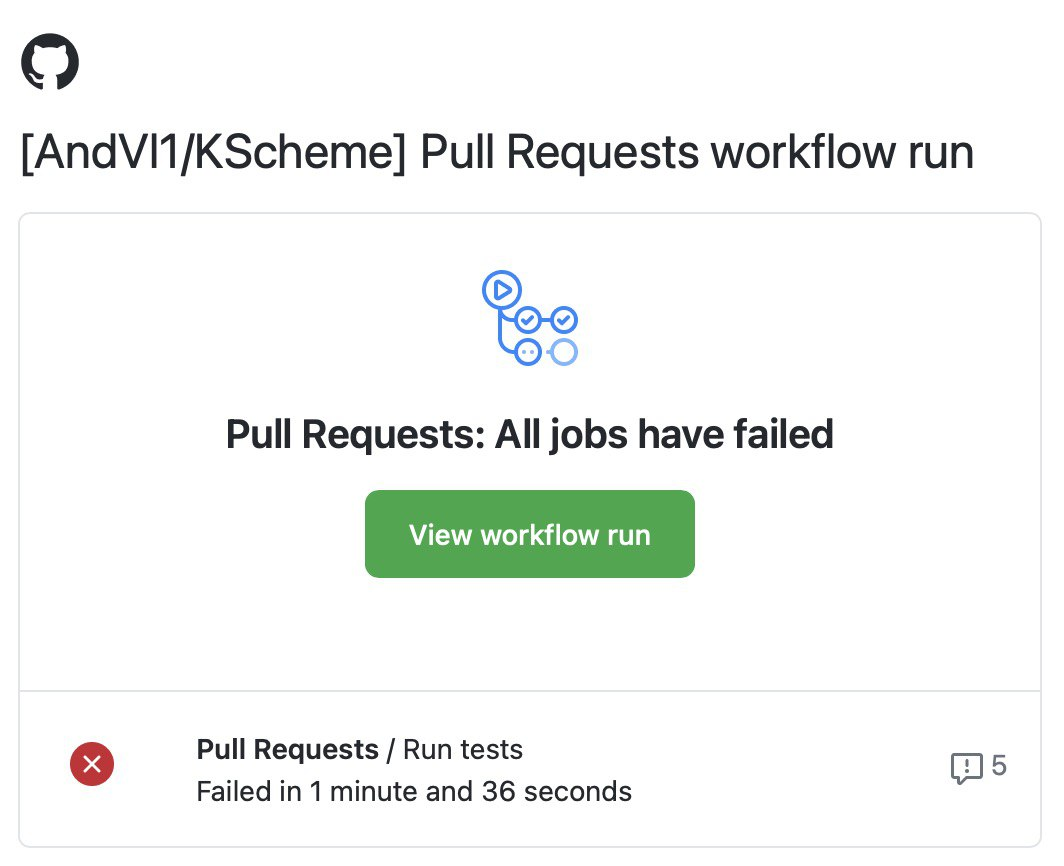
\includegraphics[width=0.5\textwidth]{fail.jpg}
\caption{Пример письма о непрохождении тестов.}
\label{fig::fail}
\end{figure}

 \anonsection{ЗАКЛЮЧЕНИЕ} %\anonsection{Заключение}

В ходе работы был создан интерпретатор подмножества R$^5$RS языка Scheme.

Программа выполняет чтение программного кода из файла или из командной строки.

Интерпретатор выполняет введённый программный код и выдаёт ответ пользвателю.

Программный код имеет много возможностей для модификации, от добавления нового функционала до написания приложений с графическим пользовательским интерфейсом для взаимодействия с интерпретатором и выполнения программного кода.

В рамках курсовой работы был написан интерпретатор языка Scheme на языке Kotlin/JVM. Интерпретатор умеет обрабатывать большую часть функций из перечисленных в стандарте R$^5$RS, тем не менее, есть достаточно большая возможность для расширения функционала.
Также есть возможность в модификации программного кода таким образом, чтобы интерпретатор можно было использовать на различных платформах для выполнения программного кода.

\renewcommand\refname{СПИСОК ИСПОЛЬЗОВАННЫХ ИСТОЧНИКОВ}
% Список литературы
\clearpage
%\bibliographystyle{ugost2008s}  %utf8gost71u.bst} %utf8gost705u} %gost2008s}
{\catcode`"\active\def"{\relax}
\addcontentsline{toc}{section}{\protect\numberline{}\refname}%
%\bibliography{biblio} %здесь ничего не меняем, кроме, возможно, имени bib-файла
\printbibliography
}
\newpage
\settocdepth{section}

\end{document}
